
\begin{questions}

\question[1] \textbf{True or False:} Recurrent neural networks (RNN's) process a time series of inputs by keeping track of separate weight vectors for each time step and applying them to the corresponding time step during inference.
    \begin{checkboxes}
     \choice True 
     \choice False
    \end{checkboxes}
    \begin{soln}
    False\\
    
    Brynn's comment: I found the wording here a bit confusing. I would probably cut this.  \\ Tom comment: I tried rewording it, as I like the question.  Is it ok now?
    \end{soln}
    \begin{qauthor}
    Input (1) Varun Natu (2) RNN Weight sharing across time steps
    \end{qauthor}
       
      
\question[1] \textbf{Select all that apply:}  Which of the following are true?
{%
    \checkboxchar{$\Box$} % change checkbox style locally
    \begin{checkboxes}
     \choice Stochastic Gradient Descent (SGD) is guaranteed to decrease the loss at every iteration
     \choice SGD reduces computational cost per update of the parameters, relative to gradient descent (GD).
     \choice SGD is parallelizable. For instance it is possible to compute the first 100 iterations simultaneously.
     \choice SGD can be used to train logistic regression and neural networks
     \choice None of the above
    \end{checkboxes}
    }
    \begin{soln}
    B, D\\
    
    Brynn's comment: for option b should we add "..relative to GD?" or something like that? \\ Matt's comment: needs to mention computational cost per update of params. Added None of the above.
    \end{soln}
    \begin{qauthor}
    Amanda Coston
    \end{qauthor}
    
    
\question[1] \textbf{True or False:} For logistic regression, higher learning rates will always converge faster during stochastic gradient descent.
    \begin{checkboxes}
     \choice True 
     \choice False
    \end{checkboxes}
    \begin{soln}
    False
    \end{soln}
    \begin{qauthor}
    (1) Daniel Min (2) Understand concept of learning rates and optimization of learning rates
    \end{qauthor}


\question[1] \textbf{True or False:} It is possible for a convolutional layer in a neural network to be converted into a linear layer (i.e., a layer whose outputs are linear functions of the inputs) and achieve the same outputs.
    \begin{checkboxes}
     \choice True 
     \choice False
    \end{checkboxes}
    \begin{soln}
    True. 
    \end{soln}
    \begin{qauthor}
    (1) Daniel Min (2) Understand underlying structure of CNN
    \end{qauthor}
    
\question[2] \textit{CNNs and parameter sharing.} Consider the following flattened representation of a convolution layer over a 3x3 image with the connections missing.
    \\ 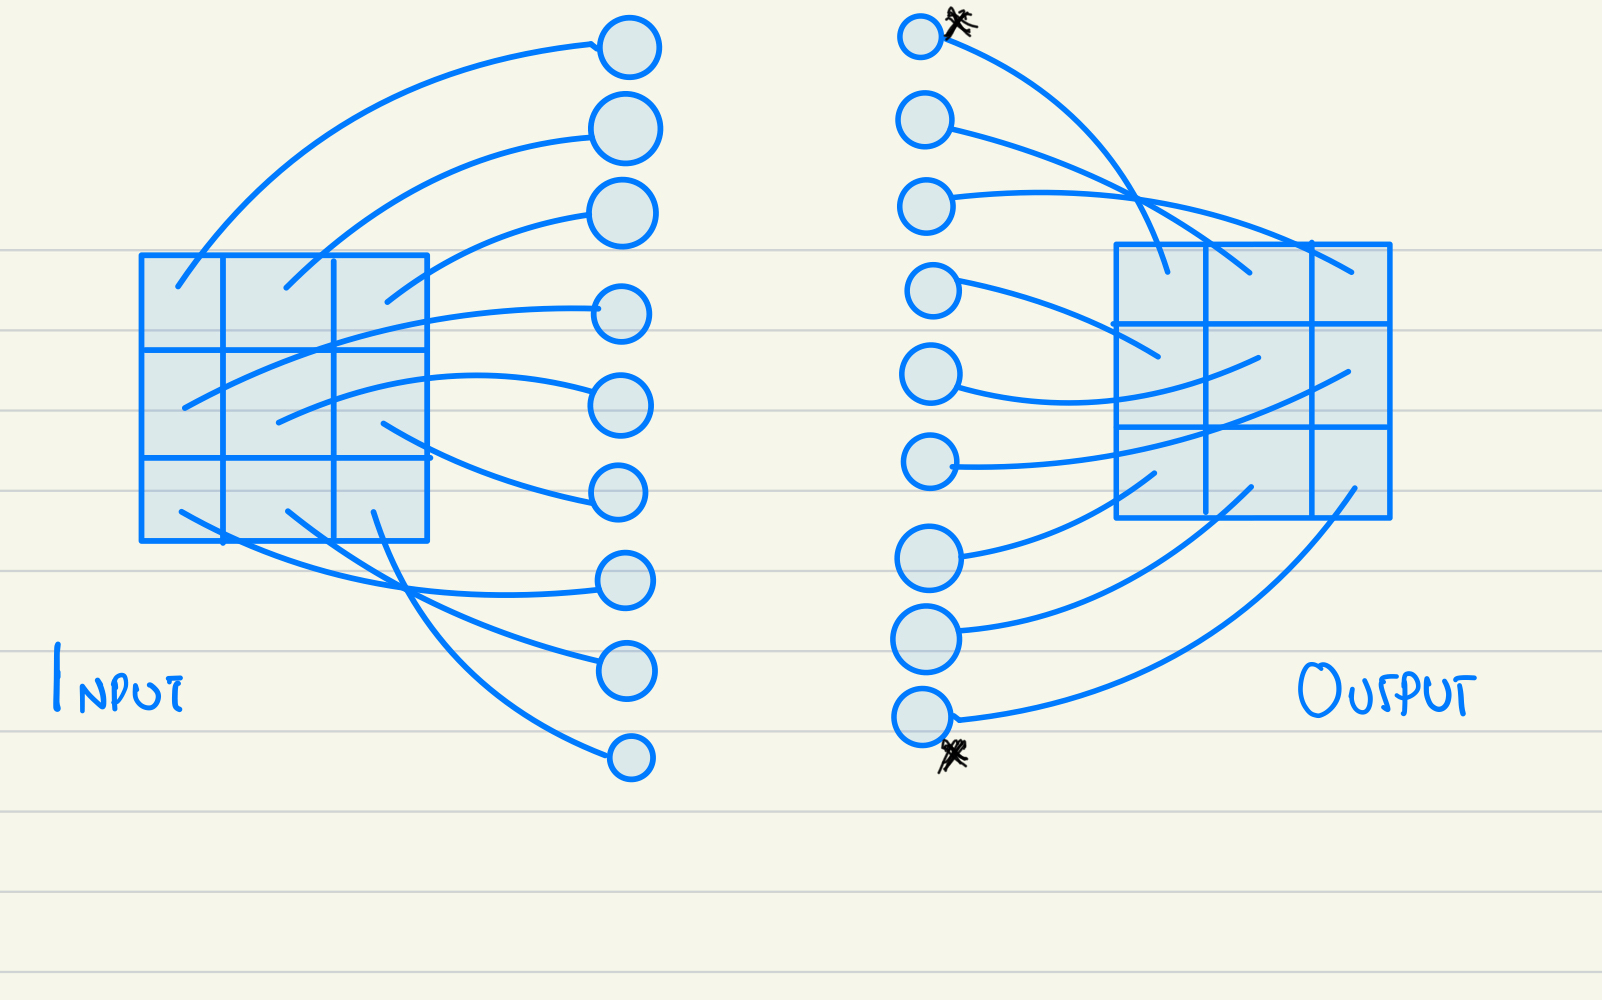
\includegraphics[width=4cm,height=4cm]{figures/CNN_flat.jpeg}
     \textbf{Numerical answer:} Given a stride of 1 and padding of 1, What should be the size of the kernel to obtain the output image ?
    \begin{tcolorbox}[fit,height=1cm, width=2cm, blank, borderline={1pt}{-2pt}]
    %solution
    \end{tcolorbox}
    \begin{soln}
    3x3
    Brynn's comment: This is ok. \\ Tom comment: I agree.
    \end{soln}

\question[1] \textbf{Select all that apply:} Which of the following is true about the convergence of policy iteration and value iteration. 
    {%
    \checkboxchar{$\Box$} % change checkbox style locally
    \begin{checkboxes}
     \choice Policy iteration can converge to an optimal policy before the state values converge.  
     \choice For large state spaces, policy iteration is more computationally expensive per iteration than value iteration.
     \choice For large action spaces, policy iteration is more computationally expensive per iteration than value iteration. 
     \choice In general, policy iteration requires fewer iterations to converge than value iteration.
     \choice None of the above.
    \end{checkboxes}
    }
    \begin{soln}
    B, D
    
    Brynn's comment: For option B should one of these be value iteration?\\
    Matt's comment: fixed wording of options. Added None of the above.
    \end{soln}
    \begin{qauthor}
    Input (1) Young Kim (2) Contrast the computational complexity and empirical convergence of value iteration vs. policy iteration
    \end{qauthor}
    

\question[1] \textbf{True or False:} Dynamic programming reinforcement learning algorithms such as policy iteration and value iteration are able to learn nonlinear functions between states and values given a finite state space.
    \begin{checkboxes}
     \choice True 
     \choice False
    \end{checkboxes}
    \begin{soln}
    True
    \end{soln}
    \begin{qauthor}
    Input (1) Young (2) Identify the conditions under which the value iteration algorithm will converge to the true value function
    \end{qauthor}
    
    
    
\question[1] \textbf{True or False:} In neural networks, the term "Transformer network" refers to any neural network that maps an input sequence to an output sequence.
    \begin{checkboxes}
     \choice True 
     \choice False
    \end{checkboxes}
    \begin{soln}
    False. Transformers are a particular neural net architecture for sequence-to-sequence problems, but there are others too.  \\
    \end{soln}
    \begin{qauthor}
    Tom
    \end{qauthor}    
    
    
\question[1] \textbf{True or False:} The term "word embeddings" refers to learned hidden layer representations of words, learned by a neural network where words are originally input using a "1-hot" encoding (i.e., an encoding with all zeros except for a single 1).
    \begin{checkboxes}
     \choice True 
     \choice False
    \end{checkboxes}
    \begin{soln}
    True.  \\
    \end{soln}
    \begin{qauthor}
    Tom
    \end{qauthor}

% Tom comment: I'm deleting this question because this semester we didn't cover skip gram models in this detail, not the defintiion of "traditional softmax."  I replaced it by the above T/F question.
%\question[1] \textbf{Numerical answer:} In the word2vec skip-gram model, if we were to use a vocabulary size of 10,000 on a corpus of 1,000,000 words with a context size of 50 and a feature size of 300, using traditional softmax, how many trainable parameters would we have?
    
\question[1] \textbf{Select all that apply:} Which of the following statements are true about L1 and L2 regularization in the context of logistic regression.
    {%
    \checkboxchar{$\Box$} % change checkbox style locally
    \begin{checkboxes}
     \choice L2 regularization restricts our parameter optimization to a convex set while L1 regularization restricts our optimization to a possibly non-convex set.
     \choice L2 regularization always leads to lower magnitude weights than L1 regularization.     
     \choice L1 regularization always leads to lower magnitude weights than L2 regularization.
     \choice Both L1 and L2 regularization prevent the weights from tending towards positive or negative infinity.
     \choice None of the above.
    \end{checkboxes}
    }
    \begin{soln}
    D only
    
    Brynn's comment: For option B--what is "more strict"?
    \\ Tom's comment: I changed option B to address this (and added option C).  Seems ok now.
    \end{soln}
    \begin{qauthor}
    Input (1) Everett Knag 
    \end{qauthor}

\end{questions}


\begin{questions}
\question[2] Design a third feature $x_3$ such that the data shown in Figure \ref{fig:feateng} is linearly separable in the higher dimensional space. (Please specify your answer in the form of an equation, i.e. $x_3 = \ldots$.)

    \begin{figure}[H]
    \begin{center}
    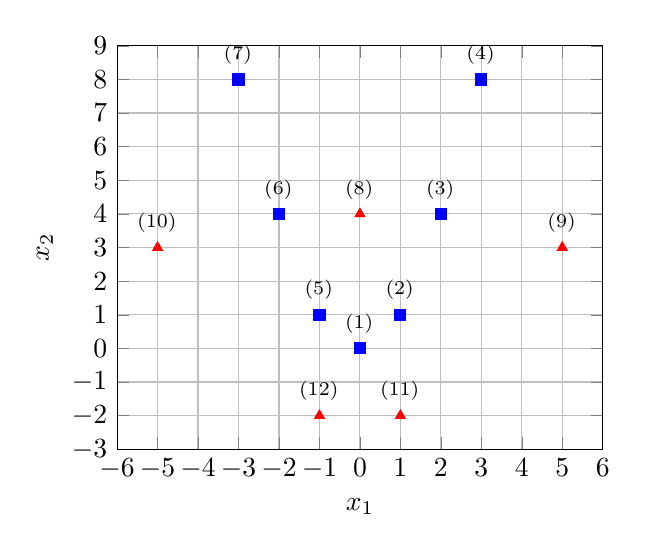
\begin{tikzpicture}
    \begin{axis}[
        scale=0.9,
        xmin=-6, xmax=6, xtick={-6,...,6},
        ymin=-3, ymax=9, ytick={-3,...,9},
        samples=50, grid=major, xlabel=$x_1$, ylabel=$x_2$]
        %\addplot[blue, ultra thick] (x,x*x);
        %\addplot[red,  ultra thick] (x*x,x);
        \addplot [
            scatter,
            only marks,
            point meta=explicit symbolic,
            scatter/classes={
                a={mark=square*,blue},
                b={mark=triangle*,red}
            },
            nodes near coords*={$\xv^{(\pgfmathprintnumber[frac]\myvalue)}$},
            visualization depends on={\thisrow{myvalue} \as \myvalue},
        ] table [meta=label] {
            x y label myvalue
            0  0 a 1
            1  1 a 2
            2  4 a 3
            3  8 a 4
            -1  1 a 5
            -2  4 a 6
            -3  8 a 7
            0 4 b 8
            5 3 b 9
            -5 3 b 10
            1 -2 b 11
            -1 -2 b 12
        };
    \end{axis}
    \end{tikzpicture}
    \end{center}
    \caption{}
    \label{fig:feateng}
    \end{figure}

    \begin{tcolorbox}[fit,height=2cm, width=15cm, blank, borderline={1pt}{-2pt}]
    %solution
    \end{tcolorbox}
    \begin{soln}
    Sample Answers 
    $$ x_3 = I (x_2 = x_1^2) $$
    $$x_3 = | x_1^2 - x_2| $$
    $$x_3 = | 2^{|x_1|} - x_2| $$
    $$x_3 \triangleq \mathbbm{1}(x_2 = 2^{|x_1|})$$
    Use Varun's script for grading this one.
    \end{soln}
    \begin{qauthor}
    Matt
    \end{qauthor}
    
\begin{EnvFullwidth}
    Your friend Harry attends Hogwarts School of Witchcraft and Wizardry, but is home visiting Pittsburgh for spring break. Harry has asked for your help on his potions homework. Professor Snape gave each student a list of 1,000 ingredients and asked them to design a potion that disguises one's appearance using at most 50 grams of each ingredient. 
    
    To speed along the process, you suggest that Harry use the potion simulator software developed by Chemical Engineering researchers at CMU to evaluate Harry's objective function. The input to the simulator is a vector of weights $\thetav$ defining a recipe, where $\theta_j \in [0, 50]$ gives the weight in grams of the $j$th ingredient. The simulator outputs $J(\thetav) \in \Rb^+$ which is the extent to which the potion formed by $\thetav$ changes one's appearance (higher is better).
    
\end{EnvFullwidth}
    
\question[2] \textbf{Short Answer:} Given that $J(\thetav)$ is a black-box simulator, design an algorithm for finding a good potion recipe $\theta$. (You may \emph{not} assume that gradient information is magically available.)
    \begin{tcolorbox}[fit,height=1cm, width=15cm, blank, borderline={1pt}{-2pt}]
    %solution
    \end{tcolorbox}
    \begin{soln}
    Valid solutions include: random search, gradient descent with finite difference approximation of $\nabla_{\thetav}J(\thetav)$
    \end{soln}
    \begin{qauthor}
    Matt
    \end{qauthor}
    
\question[2] After running your algorithm above, Harry finds that the proposed recipe $\hat{\thetav}$ would be very expensive to make since it includes a large quantity of many different expensive ingredients. Define a new objective function such that when optimized by your algorithm above, will yield a recipe which maximizes $J(\thetav)$ while keeping the total weight of all ingredients (in grams)  small.
    \begin{tcolorbox}[fit,height=1cm, width=15cm, blank, borderline={1pt}{-2pt}]
    %solution
    \end{tcolorbox}
    \begin{soln}
    Valid solutions will include a regularizer. For example,  $J'(\thetav) = J(\thetav) + \lambda r(\thetav)$ where $r(\thetav)$ is an L1 or L2 regularizer. L0 is unconventional but also technically correct.
    \end{soln}
    \begin{qauthor}
    Matt
    \end{qauthor}
    
\question[3] Harry's friend Hermione informs him that only a dozen or so ingredients are necessary. Define a new objective function that when optimized by your algorithm above, will yield a recipe which maximizes $J(\thetav)$ while keeping the number of ingredients used close to $12$, without concern for the amount of each ingredient that is included.
    \begin{tcolorbox}[fit,height=1cm, width=15cm, blank, borderline={1pt}{-2pt}]
    %solution
    \end{tcolorbox}
    \begin{soln}
    $J'(\thetav) = J(\thetav) + \lambda r(\thetav)$ where $r(\thetav) = \left| 12 - \sum_{j = 1}^{1000} \mathbbm{1}(\theta_j > 0) \right|$ 
    \end{soln}
    \begin{qauthor}
    Matt
    \end{qauthor}
    
\question[3] Hermione gives Harry a magic spell that modifies the simulator from CMU to return a single partial derivative. That is, passing a recipe $\thetav$ and an ingredient index $j$ to the simulator returns two values:
$$a, b = \text{simulator}(\thetav, j)$$
where $a = J(\thetav)$ and $b = \frac{\partial J(\thetav)}{\partial \theta_j}$. Conveniently, the spell also extends the support of $J(\cdot)$ to all vectors $\thetav \in \Rb^{1000}$ with values of $\thetav \notin [0, 50]^{1000}$ being non-optimal. Harry knows a little bit of machine learning and writes the \emph{partial} implementation of gradient ascent below.

    \begin{algorithmic}[1]
    \Procedure{GradientAscent}{}
    \State $\thetav \rightarrow 0$ \Comment{Initialize parameters to vector of all zeros} 
    \While{true}
        \State $\gv \rightarrow 0$ \Comment{Initialize a gradient vector to all zeros}
        \State \emph{[Fill in the missing lines here]}
        \If{$||\gv||_2 < \epsilon$} \Comment{Stop when gradient vector is small}
            \State \text{break}
        \EndIf
    \EndWhile
    \Return $\thetav$ \Comment{Return the best parameters}
    \EndProcedure
    \end{algorithmic}

Fill in the missing lines in order to maximize the function $J(\thetav)$. (Report only the missing lines!)

    \begin{tcolorbox}[fit,height=1cm, width=15cm, blank, borderline={1pt}{-2pt}]
    %solution
    \end{tcolorbox}
    \begin{soln}
    \begin{algorithmic}[1]
    \Procedure{GradientAscent}{}
    \State $\thetav \rightarrow 0$ \Comment{Initialize} 
    \While{true}
        \State $\gv \rightarrow 0$ \Comment{Initialize a gradient vector to all zeros}
        \For{$j \in \{1, \ldots, 1000\}$} \Comment{Loop through ingredients}
            \State $J, g_j \rightarrow \text{simulator}(\thetav, j)$ \Comment{Compute and store $j$th derivative}
        \EndFor
        \State $\thetav \rightarrow \thetav + \gamma \gv$ \Comment{Update parameters}
        \If{$||\gv||_2 < \epsilon$} \Comment{Stop when gradient vector is small}
            \State \text{break}
        \EndIf
    \EndWhile
    \Return $\thetav$ \Comment{Return the best parameters}
    \EndProcedure
    \end{algorithmic}
    \end{soln}
    \begin{qauthor}
    Matt
    \end{qauthor}
    
\question[4] Harry's friend Ron also obtains the potion simulator software for his personal laptop. Ron tries the spell from Hermione so that his copy of the simulator returns partial derivatives as well. Unfortunately, the spell goes wrong and his copy of the simulator returns two values as follows:
$$a, b = \text{simulator}(\thetav, j)$$
where $a = J(\thetav)$ and $b = \frac{\partial J(\thetav)}{\partial \theta_j} + \epsilon$ where $\epsilon \sim \text{Gaussian}(\mu = 3, \sigma^2 = 4)$. Show how to compute a vector $\gv \in \Rb^{1000}$ that equals the true gradient in expectation, i.e. that $E[\gv] = \nabla_{\thetav} J(\thetav)$.
    \begin{tcolorbox}[fit,height=1cm, width=15cm, blank, borderline={1pt}{-2pt}]
    %solution
    \end{tcolorbox}
    \begin{soln}
    For all $j \in \{1, \ldots, 1000\}$, compute $g_j = simulator(\thetav, j) - 3$.
    This is justifiable since $E[g_j] = \frac{\partial J(\thetav)}{\partial \theta_j} + E[\epsilon] - 3 = \frac{\partial J(\thetav)}{\partial \theta_j} + 3 - 3 = \frac{\partial J(\thetav)}{\partial \theta_j}$
    \end{soln}
    \begin{qauthor}
    Matt
    \end{qauthor}


\end{questions}


This question asks you to consider building neural networks out of a new type of unit, which we will call the {\em multiply-divide unit}, or MD unit.  The unit has two real-valued inputs, $x_1$ and $x_2$, and its output $o$ is equal to $f(g(x_1,x_2))$, where

\begin{itemize}
    \item $f(z) = ReLU(z) = max(0,z)$
    \item $g(x_1,x_2) = w_m x_1 x_2 + w_d \frac{x_1}{x_2}$
    \item Therefore, $o = f(g(x_1,x_2)) = max(0, w_m x_1 x_2 + w_d \frac{x_1}{x_2}) $
    \item $w_m$ and $w_d$ are the parameters to be learned
\end{itemize}

\begin{center}
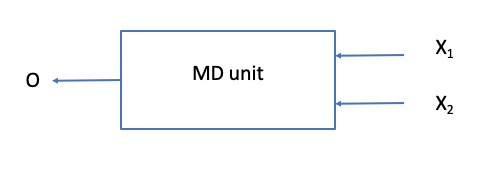
\includegraphics[width=10cm]{figures/MDunit.png}
\[ o = f(g(x_1,x_2)) = max(0, w_m x_1 x_2 + w_d \frac{x_1}{x_2}) \]
\end{center}


\begin{questions}
% \question[2] For any unit whose output is of the form $o = f(g(x_1,x_2))$ we can use the chain rule to write the derivative $\frac{\partial o}{\partial x_1}$ as the product of two other derivatives.  Write that product here. (Report only your final answer, not your work.)

\question[2] \textbf{Select one:} Consider a unit whose output is of the form $o = f(g(x_1,x_2))$. If possible, use the chain rule to write the derivative $\frac{\partial o}{\partial x_1}$ as the product of two other derivatives.
    \begin{checkboxes}
     \choice $\frac{\partial o}{\partial g}\frac{\partial g}{\partial x_2}$
     \choice $\frac{\partial o}{\partial g}\frac{\partial g}{\partial x_1}$
     \choice $\frac{\partial o}{\partial f}\frac{\partial f}{\partial x_1}$
     \choice We cannot write $\frac{\partial o}{\partial x_1}$ as a product of other derivatives.
    \end{checkboxes}
    \begin{soln}
    (b)
    \end{soln}
\vspace{1 in}

% \question[2] Now consider our MD unit.  To train it using gradient descent, we will need to know the partial derivatives $\frac{\partial o}{\partial w_m}$ and $\frac{\partial o}{\partial w_d}$. Write the expression for $\frac{\partial o}{\partial w_m}$.  Your expression should be in terms of (some subset of) $o, x_1, x_2, w_m$ and $w_d$.  You may write this as an if statement if you like. (Report only your final answer, not your work.)

\question[2] \textbf{Select one:} Now consider our MD unit.  To train it using gradient descent, we will need to know the partial derivatives $\frac{\partial o}{\partial w_m}$ and $\frac{\partial o}{\partial w_d}$. Choose the expression for $\frac{\partial o}{\partial w_m}$.
    \begin{checkboxes}
     \choice $\begin{cases}x_1x_2 &\text{if $w_mx_1x_2 \ge 0$}\\
     0 &\text{if $w_mx_1x_2 < 0$}
     \end{cases}$
     \choice $\begin{cases}x_1x_2 &\text{if $w_mx_1x_2+w_d\frac{x_1}{x_2}\ge 0$}\\
     0 &\text{if $w_mx_1x_2+w_d\frac{x_1}{x_2}< 0$}
     \end{cases}$
     \choice$\begin{cases}\frac{x_1}{x_2} &\text{if $w_mx_1x_2+w_d\frac{x_1}{x_2}\ge 0$}\\
     0 &\text{if $w_mx_1x_2+w_d\frac{x_1}{x_2}< 0$}
     \end{cases}$
     \choice $\begin{cases}\frac{x_1}{x_2} &\text{if $w_mx_1x_2\geq 0$}\\
     0 &\text{if $w_mx_1x_2 < 0$}
     \end{cases}$
    \end{checkboxes}
    \begin{soln}
    (b)
    \end{soln}


\vspace{1 in}



\fullwidth{Now consider a two-layer network of MD units as shown in the figure below. Now that we have 3 different MD Units, we will use $w_{m,i}$ to refer to the $w_m$ weight of MD unit $i$, and use $w_{d,i}$ to refer to the $w_d$ weight of MD unit $i,i=1,2,3$.

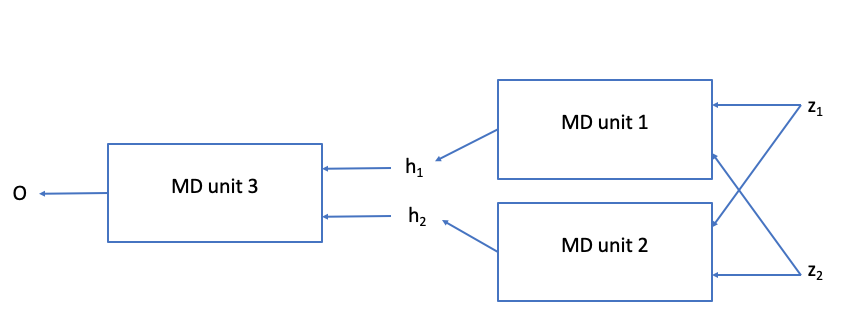
\includegraphics[width=12cm]{figures/MDunitNetwork.png} 
}

\question[1]\textbf{Select one:}
Choose the correct expression for $\frac{\partial o}{\partial h_1}$.
\begin{checkboxes}
     \choice $\begin{cases} 
     w_{m,2}z_2 &\text{if $w_{m,2}z_2 \geq 0$}\\
     0 &\text{otherwise}
    \end{cases}$
     
     \choice $\begin{cases} 
     w_{m,3} h_2 +\frac{w_{d,3}}{h_2} &\text{if $w_{m,3} h_1 h_2 +w_{d,3} \frac{h_1}{h_2} \geq 0$}\\
     0 &\text{otherwise}
    \end{cases}$
     
     \choice $\begin{cases} 
     w_{m,2} h_2 +\frac{w_{d,2}}{h_2} &\text{if $w_{m,2} h_1 h_2 +w_{d,2} \frac{h_1}{h_2} < 0$}\\
     0 &\text{otherwise}
    \end{cases}$
     
     \choice $\begin{cases} 
     w_{m,3} h_2 &\text{if $w_{m,3} h_1 h_2 +w_{d,3} \frac{h_1}{h_2} \geq 0$}\\
     0 &\text{otherwise}
    \end{cases}$
    \end{checkboxes}

\begin{soln}
(d)
\end{soln}
% \question[4]
%  Write an expression for $\frac{\partial o}{\partial w_{m,1}}$. You may write this as an if statement if you like. (Report only your final answer, not your work.)
\vspace{1 in}

\question[4]\textbf{Select one:}
Choose the correct expression for $\frac{\partial o}{\partial w_{m,1}}$.
\begin{checkboxes}
     \choice $\begin{cases}
     \frac{\partial o}{\partial h_1}z_1z_2 &\text{if $w_{m,2} z_1 z_2 +w_{d,2} \frac{z_1}{z_2} \geq 0$}\\
     0 &\text{otherwise}
     \end{cases}$
     
     \choice $\begin{cases}
     \frac{\partial o}{\partial h_1}z_1z_2 &\text{if $w_{m,1} z_1 z_2 +w_{d,1} \frac{z_1}{z_2} \geq 0$}\\
     0 &\text{otherwise}
     \end{cases}$
     
     \choice $\begin{cases}
     \frac{\partial o}{\partial h_1}\frac{z_1}{z_2} &\text{if $w_{m,2} z_1 z_2 +w_{d,2} \frac{z_1}{z_2} \geq 0$}\\
     0 &\text{otherwise}
     \end{cases}$
     
     \choice $\begin{cases}
     \frac{\partial o}{\partial h_1} &\text{if $w_{m,2} z_1 z_2 +w_{d,2} \frac{z_1}{z_2} \geq 0$}\\
     0 &\text{otherwise}
     \end{cases}$
\end{checkboxes}

\begin{soln}
(b)
\end{soln}



\end{questions}